\documentclass{article}
\usepackage[a4paper, total={7in, 9in}]{geometry}
\usepackage[brazil,portuges]{babel}
\usepackage[utf8]{inputenc}
\usepackage[T1]{fontenc}
\usepackage{ebgaramond}
\usepackage{amsmath}
\usepackage{indentfirst}
\usepackage{titlesec}
\usepackage{todonotes}
\usepackage{enumitem}
\usepackage{tikz}
\usepackage{listings}% http://ctan.org/pkg/listings
\lstset{
  basicstyle=\ttfamily,
  mathescape
}

\title{Compiladores - Exercício 5}
\author{André L. Mendes Fakhoury\\
Gustavo V. V. Silva Soares\\
Eduardo Dias Pennone\\
Matheus S. Populim\\
Thiago Preischadt\\
}
\date{2021}

\begin{document}

\maketitle

\section{A gramática a seguir, no formato BNF, é LL(1)? Se não é, transforme-a. Considere <S> como símbolo inicial da gramática.}

\begin{verbatim}
<S> ::= i<A>
<A> ::= :=<E>
<E> ::= <T> + <E> | <T>
<T> ::= <F> * <T> | <F>
<F> ::= <P> <F> | <P>
<P> ::= i | (<E>)
\end{verbatim}

A gramática acima não é LL(1). No entanto, podemos convertê-la para LL(1), como representado abaixo:

\begin{lstlisting}
S ::= i A
A ::= := E
E ::= T D
D ::= + T D
D ::= $\lambda$
T ::= F M
M ::= * F M
M ::= $\lambda$
F ::= i
F ::= ( E )
\end{lstlisting}
A -> Equ\textbf{A}ção\\
E -> \textbf{E}xpressão\\ 
T -> \textbf{T}ermo\\
D -> A\textbf{D}iciona mais um termo\\
F -> \textbf{F}ator\\
M -> \textbf{M}ultiplica mais um fator\\
i -> símbolo terminal\\
$\lambda$ -> string vazia 
\newpage

\section{Criar os grafos sintáticos relativos à gramática abaixo e o conjunto de procedimentos sintáticos para realizar a ASD preditiva recursiva}

\begin{lstlisting}
<A> ::= x | (<B>)
<B> ::= <A><C>
<C> ::= +<A><C> | $\lambda$
\end{lstlisting}

Para cada símbolo não terminal, podemos descrever os grafos sintáticos e o respectivo conjunto de procedimentos.

\begin{figure}[ht!]
    \centering
    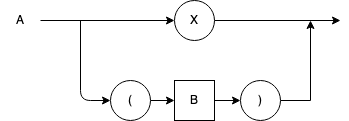
\includegraphics[width=0.5\textwidth]{ex5/A.png}
\end{figure}

\begin{verbatim}
procedimento A
begin
  se (símbolo = `x') então
    obter_símbolo;
  senão se (símbolo = `(') então
    obter_símbolo;
    B;
    se (símbolo = `)') então
      obter_símbolo;
    senão ERRO;
  senão ERRO;
end
\end{verbatim}

\begin{figure}[ht!]
    \centering
    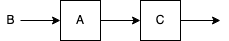
\includegraphics[width=0.3\textwidth]{ex5/B.png}
\end{figure}

\begin{verbatim}
procedimento B
begin
  A;
  C;
end
\end{verbatim}

\begin{figure}[ht!]
    \centering
    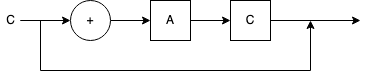
\includegraphics[width=0.5\textwidth]{ex5/C.png}
\end{figure}

\begin{verbatim}
procedimento C
begin
  se (símbolo = `+') então
    obter_símbolo;
    A;
    C;
end
\end{verbatim}



\end{document}
